%!TEX root = ../main.tex

\subsection{Tarefa de Aprendizado}
% diferenciar a métrica para cenários balanceados e desbalanceados

\begin{figure}[h!]
\centering
\caption{Uma visão geral do processo de aprendizado.}
\label{fig:esquema-solucao}
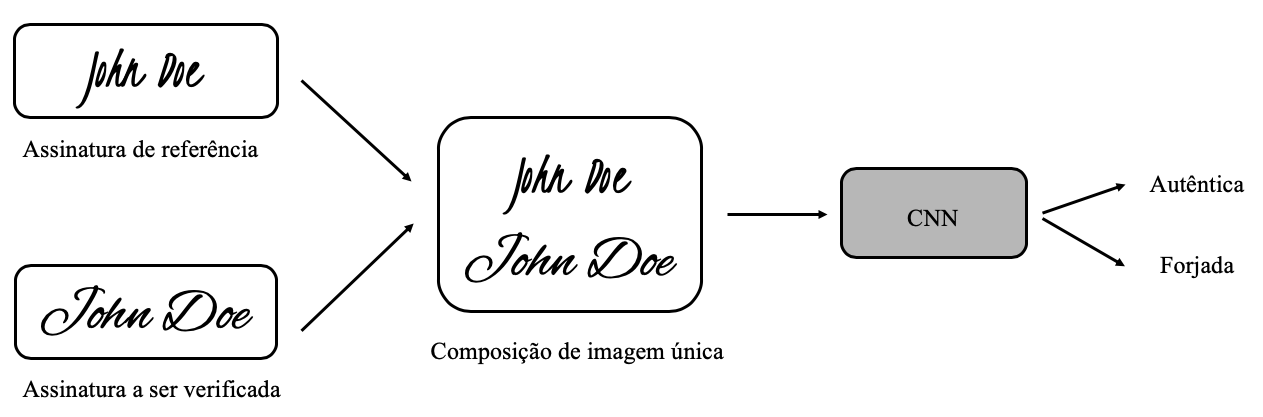
\includegraphics[width=\textwidth]{imgs/esquema-solucao}
\end{figure}

O treinamento e testes das CNNs seguirão o comportamento \emph{holdout} de validação
cruzada, em que $70\%$ dos dados serão utilizados no treino e ajuste de parâmetros e o
restante para avaliação, com vista a capturar a qualidade da generalização proposta pelos
modelos considerados.

\subsection{Visão Geral do Conjunto de Dados}
% estatisticas calculadas lá no notebook
Para a obtenção de um modelo inteligente capaz de verificar a autenticidade de assinaturas de indivíduos, é necessário, primeiramente, treiná-lo. Para tanto, é necessário um conjunto de exemplos, isto é, uma base de dados  que possua exemplos de assinaturas e seus respectivos rótulos, isto é, quando são forjadas ou genuínas, com vistas a prover características relevantes para o aprendizado.

Para este fim, utilizou-se dois conjuntos de dados originalmente disponibilizados pela
\emph{Signature Verification Competition} realizada na \emph{International Conference on Document Analysis and Recognition} em 2009. Na ocasião da competição, cada um destes conjuntos de dados foi utilizado em uma etapa. Na etapa de treinamento, foi utilizado o conjunto de assinaturas do \emph{Norwegian Information Security laboratory and Donders Centre for Cognition} (NISDCC), composto originalmente de 1.920 assinaturas genuínas e forjadas. Para a etapa seguinte, de validação dos modelos submetidos, foi utilizado o conjunto coletado pelo \emph{Netherlands Forensic Institute} (NFI), composto por 1.953 novas assinaturas genuínas e forjadas \cite{icdar2009}. Considerando que a competição ocorreu há uma década, as bases de dados utilizadas na época são atualmente mantidas pela \emph{International Association for Pattern Recognition} (IAPR) e contam com um número de 1.898 assinaturas do conjunto NISDCC e 1.564 assinaturas do conjunto NFI \cite{iapr-tc11}. Esta versão mais recente é amplamente disponibilizada e, por essa razão, está sendo utilizada no escopo deste trabalho.

Os conjuntos disponibilizados pelo IAPR são compostos por dois tipos de assinaturas, as assinaturas \emph{offline} e as assinaturas \emph{online}. Nas assinaturas \emph{offline}, é considerado apenas o aspecto estático da mesma, ou seja, uma imagem obtida após o processo da assinatura ter sido concluído. Estes dados foram segmentados, inspecionados visualmente e, em seguida, pré-processados para fornecer imagens formatadas em cores, em escala de cinza e binárias com a resolução de $600$ dpi. Os dados das assinaturas \emph{online}, por sua vez, continham informações dinâmicas, que consistiam em arquivos de texto que descreviam os detalhes capturados em vários pontos durante o processo da assinatura, sendo estes as coordenadas $x$ e $y$ da ponta da caneta, a pressão exercida sobre a caneta, o ângulo azimutal e o ângulo de elevação \cite{icdar2009}. Um exemplo de uma assinatura \emph{offline} e a sua respectiva representação \emph{online} com os pontos plotados pode ser encontrada na Figura \ref{fig:sample-signature}.


\begin{figure}[h!]
\centering
\caption{Uma amostra das assinaturas \emph{offline} e \emph{online} do SigComp2009. Fonte: \cite{icdar2009}.}
\label{fig:sample-signature}
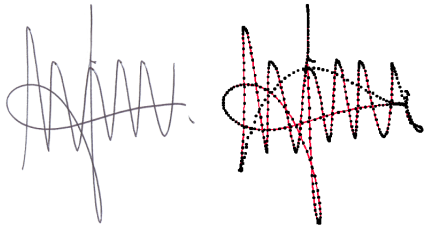
\includegraphics[width=0.5\textwidth]{imgs/sample-signature}
\end{figure}

Nestas bases de dados um certo autor produz várias versões de sua própria assinatura, compondo os exemplos de assinaturas genuínas. Várias pessoas foram convocadas a falsificar esta assinatura, produzindo os exemplos forjados das mesmas. Nestas falsificações utilizou-se a técnica \emph{over-the-shoulder}, na qual o autor forjador tem a oportunidade de visualizar a assinatura genuína antes da falsificação, podendo, inclusive, ter praticado anteriormente diversas vezes. Segundo Blankers et al., este tipo de falsificação costuma ser de difícil detecção \cite{icdar2009}.

Considerando a demanda por equipamentos específicos para obtenção das assinaturas \emph{online} e da pouca existência dos mesmos em cenários práticos, optou-se apenas pela utilização das assinaturas \emph{offline} para a elaboração deste trabalho, com vistas a concentrar os esforços em uma solução que incorpore aspectos de Visão Computacional. Após a exclusão destes exemplos, o quantitativo remanescente de assinaturas e seus tipos (genuína ou forjada) encontram-se disponíveis na Tabela \ref{tab:demonstracao-dataset}.

\begin{table}[h!]
	\centering
	\caption{Quantitativo de indivíduos e assinaturas \emph{offline} por conjunto de dados.}
	\label{tab:demonstracao-dataset}
\resizebox{\textwidth}{!}{
	\begin{tabular}{c C{2cm} C{2cm} C{3.25cm} C{2.5cm} C{2.5cm} C{2.25cm}}
		\toprule
		 \textbf{Conjunto}& \textbf{Autores originais} & \textbf{Autores forjadores} & \textbf{Autores originais com assinaturas forjadas} & \textbf{Assinaturas genuínas}  & \textbf{Assinaturas forjadas} & \textbf{Total de assinaturas} \\
		\midrule
		NISDCC & 12 & 31 & 12 & 60 & 1.838 & 1.898 \\
    NFI & 79 & 33 & 19 & 940 & 624 & 1.564 \\
		\bottomrule
	\end{tabular}}
\end{table}

Conforme pode ser observado, um mesmo autor produziu diferentes versões de sua assinatura. A coluna ``Autores originais'' indica o quantitativo destes indivíduos e a coluna ``Assinaturas genuínas'' indica o total de assinaturas feitas pelos mesmos. No caso do \emph{dataset} NISDCC, em especial, cada autor reproduziu sua própria assinatura $5$ vezes. No NFI não houve uma consistência quantitativa, mas, em média, existem $11$ reproduções da assinatura original pelo autor verdadeiro.

Ainda conforme a Tabela \ref{tab:demonstracao-dataset}, o NISDCC conta com $31$ autores forjadores, os quais produziram versões forjadas de todas as assinaturas originais, mas com um quantitativo de falsificações distintos para cada original, totalizando $1.838$ assinaturas forjadas com a técnica \emph{over-the-shoulder}. No caso do NFI, isto não ocorreu de mesma forma, pois apenas um subconjunto das originais foi alvo de falsificação.

Considerando o total exposto de assinaturas originais e forjadas, tendo sido compreendida a estrutura, organização e exemplos dos \emph{datasets}, partiu-se então para sua preparação com vistas a adequar seu uso para a solução proposta.


\subsection{Preparação do Conjunto de Dados}
Sabe-se que algoritmos de AM necessitam de quantidade significantiva de dados, preferencialmente sem muitos ruídos, para serem utilizados de forma a obter um modelo que possua bom desempenho \cite{marsland}. Levando isto em conta e com vistas a adequar os dados disponíveis com a tarefa de aprendizado considerada, uma etapa de pré-processamento fez-se necessárias, cujos passos são descritos a seguir.

Primeiramente foi necessário realizar a adaptação das imagens individuais para as imagens compostas, conforme apresentado anteriormente no esquema da Figura \ref{fig:esquema-solucao}. Para isto, foi feita a combinação de cada assinatura genuína de um autor com suas diferentes versões originais, produzindo uma nova imagem para cada caso a qual associou-se o rótulo de autêntica. Após esta etapa, também foram combinados os exemplos genuínos com suas respectivas versões forjadas, aos quais foi associado o rótulo de forjado. Todas as imagens obtidas dessas combinações serão utilizadas como exemplos para o processo de treinamento, validação e teste do modelo proposto.

O processo de combinação das imagens de cada um dos exemplos foi realizado em três etapas. Na primeira etapa, ambas as imagens foram redimensionadas para um tamanho de $256 \times 256$ \emph{pixels}. Em seguida, as imagens foram concatenadas verticalmente com a intenção de formar uma única imagem de $256 \times 512$ \emph{pixels}. Por fim, a imagem resultante foi redimensionada novamente em um tamanho de $256 \times 256$ \emph{pixels} e transformada para um espaço de cores em escala de cinza, com a intenção de padronizar todas os exemplos.

% Escrever algo sobre como foi atingida a quantidade de exemplos atual?

Ao concluir a etapa anterior, percebeu-se uma desproporção significativa no número de exemplos de cada classe, o que poderia comprometer o processo de aprendizado do modelo. Para contornar este problema, foram então consideradas três abordagens distintas para os exemplos disponíveis:

\begin{enumerate}
	\item \textbf{Abordagem 1}. Considera apenas os exemplos autênticos para os quais há uma versão forjada. Neste cenário, tem-se apenas $15\%$ de exemplos autênticos e $85\%$ de exemplos forjados;
	\item \textbf{Abordagem 2}. Nesta abordagem foi preservado o total de exemplos autênticos da abordagem anterior, mas o excedente de exemplos forjados que causavam um desbalanceamento evidente foram descartados de maneira pseudo-aleatória. Embora contenha menos exemplos, esta abordagem tem um \emph{dataset} balanceado, com mesma proporção para ambas as classes;
	\item \textbf{Abordagem 3}. Visando um melhor aproveitamento das assinaturas originais no \emph{dataset} NFI, considerou o incremento de assinaturas autênticas, ainda que não haja exemplos forjados para mesma. É importante enfatizar que os exemplos forjados desta abordagem são iguais ao da primeira. Obteve-se, então, um \emph{dataset} com mais exemplos e \emph{quasi}-balanceado.
\end{enumerate}

Após a organização dos exemplos conforme as abordagens distintas, realizou-se então a partição \emph{holdout} de validação cruzada, com $70\%$ dos exemplos para treinamento, $10\%$ para validação e $20\%$ para testes. A Tabela \ref{tab:divisao-dados} apresenta a descrição destes dados, suas quantidades e divisões e a Figura \ref{fig:divisao-dados} auxilia na visualização da proporcionalidade nas diferentes abordagens consideradas.

\begin{table}[h!]
	\centering
	\caption{Quantitativo de exemplos por abordagem, classe e finalidade na tarefa de aprendizado considerada.}
	\label{tab:divisao-dados}
\resizebox{\textwidth}{!}{
	\begin{tabular}{c c c c c c c c}
		\toprule
		\textbf{Abordagem} & \textbf{Característica} & \textbf{Tipo de Exemplo} & \textbf{Treino} & \textbf{Validação} & \textbf{Teste} & \textbf{Total} & \textbf{Proporção}\\
		\midrule
		\multirow{2}{*}{1} & \multirow{2}{*}{Dados desbalanceados} & Genuíno & 2.011 & 299 & 618 & 2.928 & $15\%$ \\
    &  & Forjado & 11.649 & 1.648 & 3.237 & 16.534 & $85\%$\\
     \midrule
    \multirow{2}{*}{2} & \multirow{2}{*}{Dados balanceados} & Genuíno & 2.011 & 299 & 618 & 2.928 & $50\%$  \\
    &  & Forjado & 2.024 & 308 & 569 & 2.901 & $50\%$ \\
		 \midrule
		\multirow{2}{*}{3} & \multirow{2}{*}{Dados \emph{quasi}-balanceados} & Genuíno & 8.131 & 1.134 & 2.257  & 11.522 & $41\%$\\
		 & & Forjado & 11.649 & 1.648 & 3.237 & 16.534 & $59\%$\\
		\bottomrule
	\end{tabular}}
\end{table}

\begin{figure}[h!]
	\centering
	\caption{Representação gráfica da proporção dos exemplos por abordagem, classe e finalidade na tarefa de aprendizado considerada.}
	\subfloat[Abordagem 1\label{subfig:approach1}]{%
	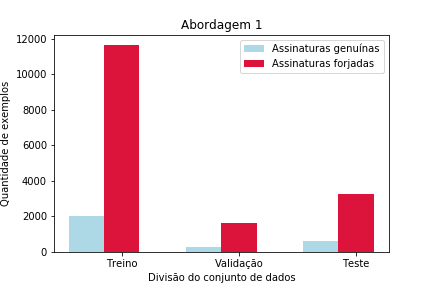
\includegraphics[width=0.5\textwidth]{imgs/approach1}
	}
	\subfloat[Abordagem 2\label{subfig:approach2}]{%
	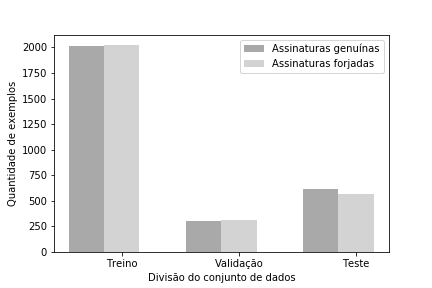
\includegraphics[width=0.5\textwidth]{imgs/approach2}
	}
	\hfill
	\subfloat[Abordagem 3\label{subfig:approach3}]{%
	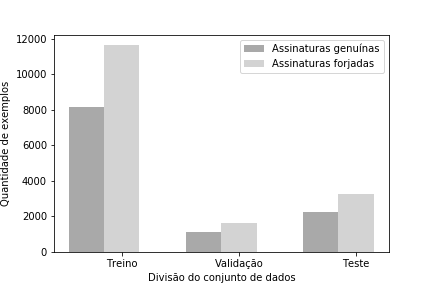
\includegraphics[width=0.5\textwidth]{imgs/approach3}
	}
	\label{fig:divisao-dados}
\end{figure}

Ao serem fornecidas para treinamento pelas CNNs, todas os \emph{pixels} das imagens serão normalizados por meio de uma divisão por $255$, passando a residirem no intervalo $[0,1]$. Esta normalização é realizada em virtude das redes neurais que, em geral, aprendem mais eficientemente nestas condições \cite{chollet}.


\subsection{Modelos, Parâmetros e Hiperparâmetros Considerados}
